\documentclass[a4paper,english]{article}

\usepackage[dvips]{graphicx}
\usepackage[top=2cm,bottom=3cm,left=1.5cm,right=1.5cm]{geometry}
\usepackage{amsmath}
\usepackage{subfigure}

\title{Machine Intelligence 2 \\ Exercise sheet 9}
\author{Group 1 \\Tiziano, Raphael, Stephan}
\date{\today}
\begin{document}
\maketitle


\section*{Exercise 1 - Simulated Annealing}
We applied simulated annealing to find the state of the network associated to the minimum energy. We run the algorithm with the following parameters: $\beta = 0.1,
\tau = 1.1, t_{max} = 100$. The algorithm converged to a minimum after 4 iterations. Figure~\ref{et} shows the evolution of the energy function and of the temperature over time.
In Figure~\ref{bar} we plot the energy value and the associated probability for each possible state of the network (for different values of the parameter $\beta$). From the energy distribution we can see that the algorithm converged to a global optimum (minimum energy). From the probability distributions we can observe that states with lower energies are associated to higher probabilities and that probability distributions become more ``peaky" increasing the value of $\beta$. This means that increasing $\beta$ over time we have an higher and higher probability to remain in a minimum of the energy function. 

\begin{figure}[h!]
\centering
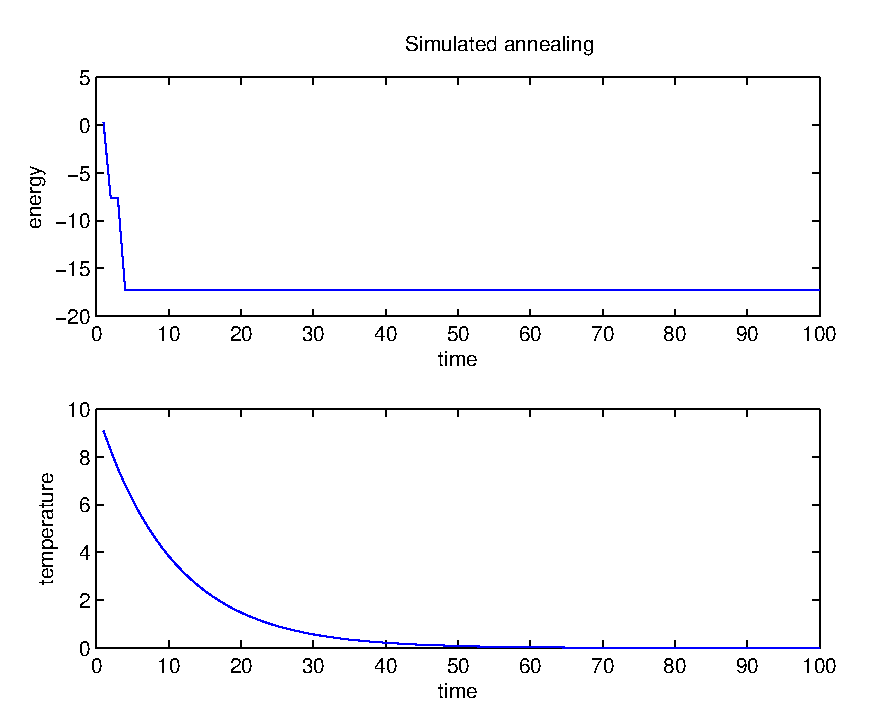
\includegraphics[scale = .7]{ex1_annealing_et.eps}
\caption{Evolution of the total energy function of the network and of the temperature over time during simulated annealing. Convergence is reached after 4 iterations}
\label{et}
\end{figure}


\begin{figure}[h!]
\centering
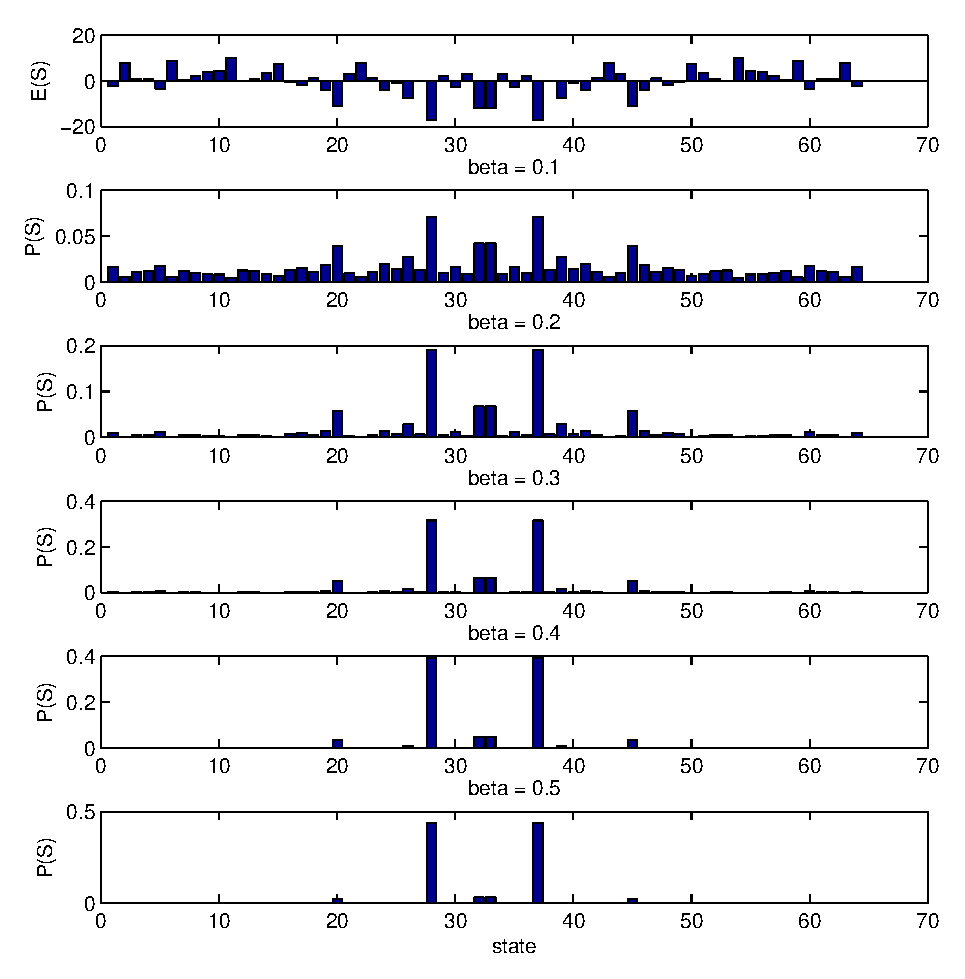
\includegraphics[scale = 1]{ex1_annealing_bar.eps}
\caption{Energy value [Top] and associated probability for each possible state of the network. The probability function has been evaluated for different values of the annealing parameter $\beta$.}
\label{bar}
\end{figure}

\clearpage
\section*{Exercise 2 - Mean-Field Annealing}
We applied mean-field annealing to the same optimization problem in Exercise 1. We run the algorithm with the same parameters ($\beta = 0.1, \tau = 1.1, t_{max} = 100$) and we started from the same initial state in order to compare the results. Figure \ref{mf_et} shows the evolution of the energy function and of the temperature over time. The algorithm converges to a global optimum but  we observe that the energy function changes more smoothly and it takes an higher number of iterations (30) in order to reach convergence. However we cannot exclude that in a more complex optimization problem mean-field annealing could outperform simulated annealing in terms of convergence time. 

\begin{figure}[h!]
\centering
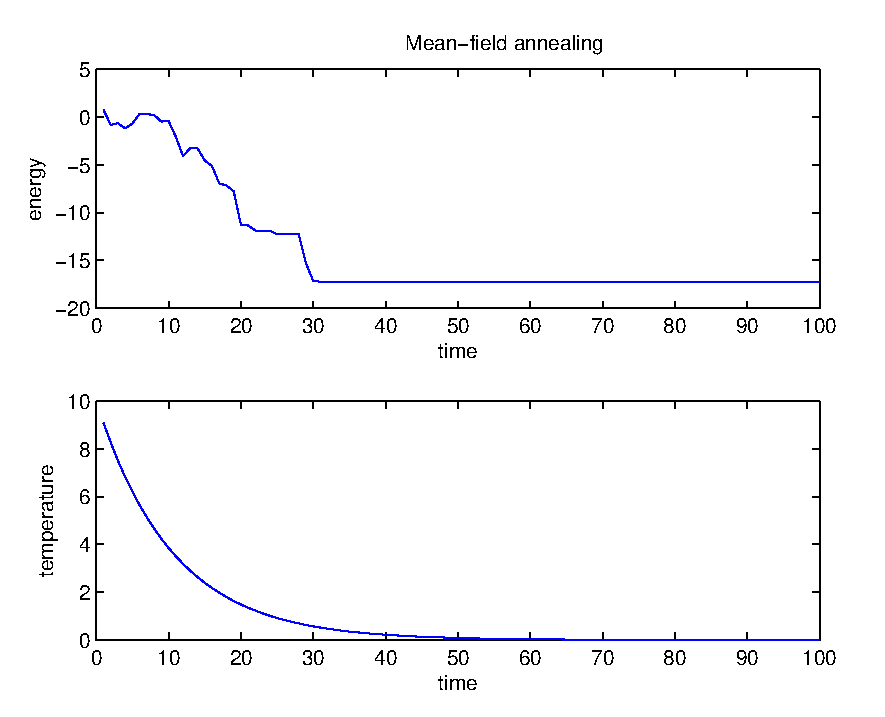
\includegraphics[scale = .7]{ex2_mean_fields_et.eps}
\caption{Evolution of the total energy function of the network and of the temperature over time during mean-field annealing. Convergence is reached after 30 iterations}
\label{mf_et}
\end{figure}

\clearpage
\section*{Exercise 3 - Online K-means clustering}
We implemented online K-means clustering with the suggested annealing schedule and using the following parameters $K  = 4, \eta  = 0.3, \tau = 0.8$.
Figure~\ref{km_steps} shows the evolution of the prototypes' positions during the algorithm, while Figure~\ref{km_err} shows the evolution of the error function over time.
The algorithm converges after approximately 100 iterations and when convergence is reached the error function reaches its minimum.

\begin{figure}[h!]
\centering
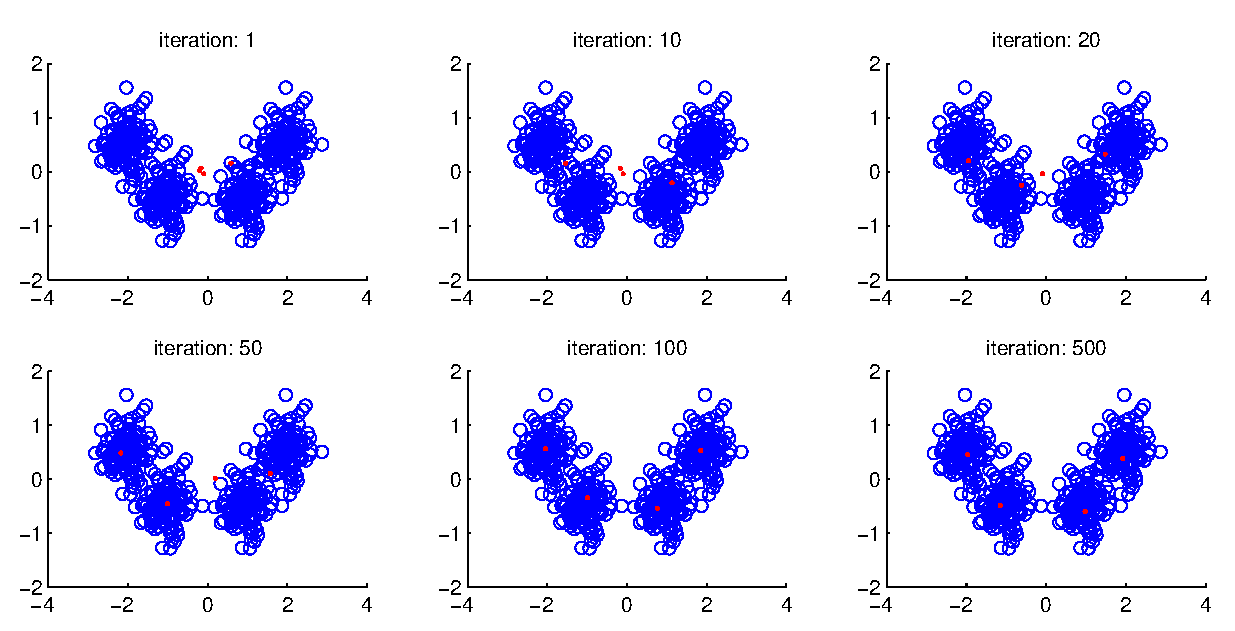
\includegraphics[scale = 0.8]{ex3_kmeans_steps}
\caption{Online k-means at different iterations. Data is plotted in blue, while prototypes are marked in red.}
\label{km_steps}
\end{figure}

\begin{figure}[h!]
\centering
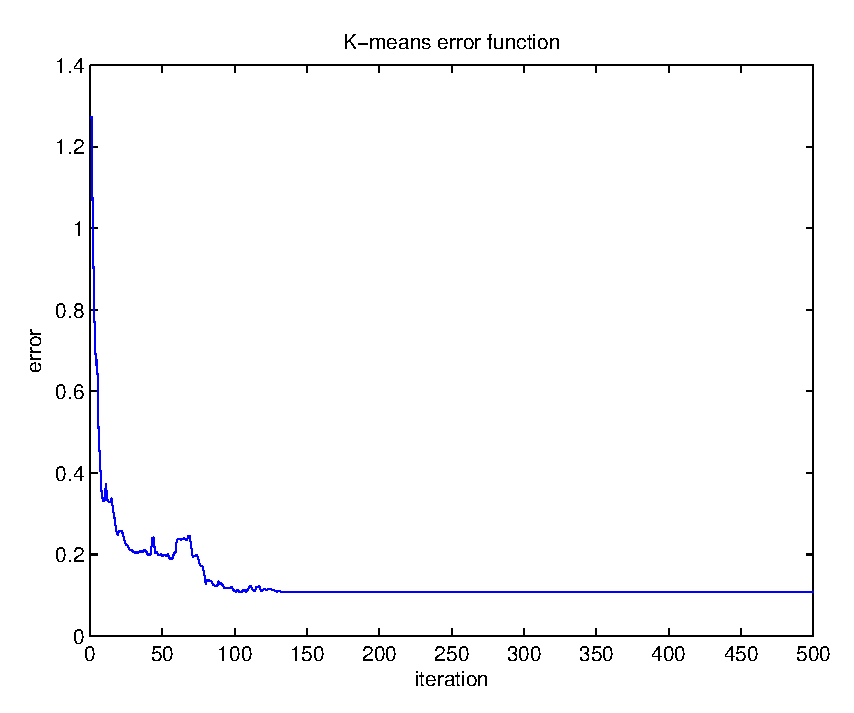
\includegraphics[scale = 0.6]{ex3_kmeans_error}
\caption{Energy value [Top] and associated probability for each possible state of the network. The probability function has been evaluated for different values of the annealing parameter $\beta$.}
\label{km_err}
\end{figure}

\clearpage
\section*{Exercise 4 - Soft K-means clustering}
We implemented soft K-means clustering in two versions: 
\begin{itemize}
\item with K=8 and no annealing (fixed values of $\beta$);
\item with K = 4,6,8 and an annealing schedule.
\end{itemize}
In both versions we used a convergence criterion $\gamma = 0.01$.
Figure~\ref{soft_km} shows the results obtained for the first implementation of the algorithm. Increasing the parameter $\beta$ the prototypes start to move away from their initial position toward the  centers of the clusters. For $\beta < 1$ the prototypes are all clustered together, at about $\beta = 1$ they form two clusters, at $\beta = 2$ they form 4 clusters and finally when $\beta$ is approximately 15 they split in 8 clusters. Observing that we have 4 clusters for a very large range of $\beta$ it might be also possible to infer the optimal number of clusters directly from data.
 
\begin{figure}[h!]
%\centering
\subfigure[]{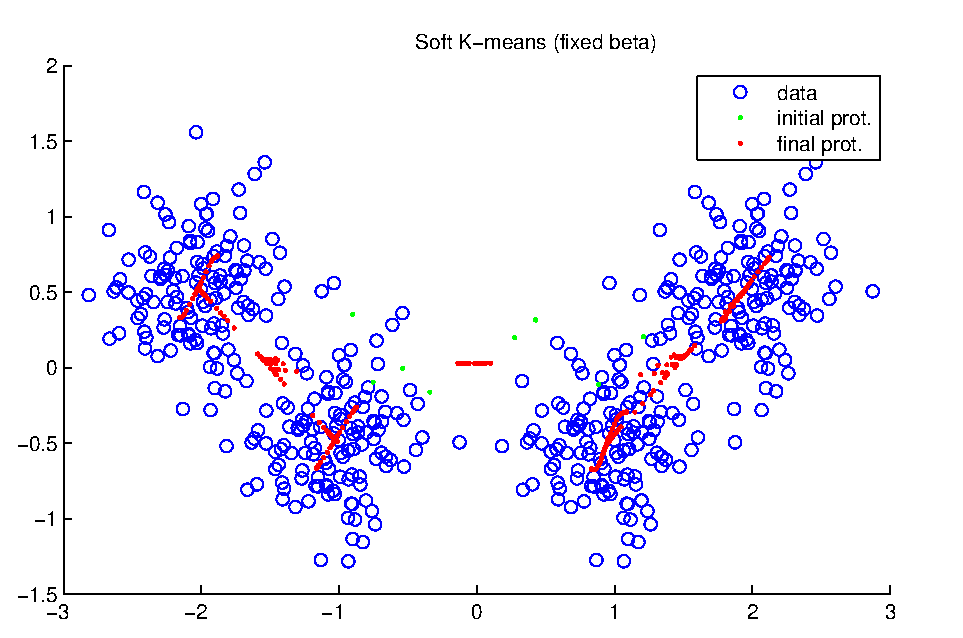
\includegraphics[scale = 0.55]{ex4_soft_kmeans}}
\subfigure[]{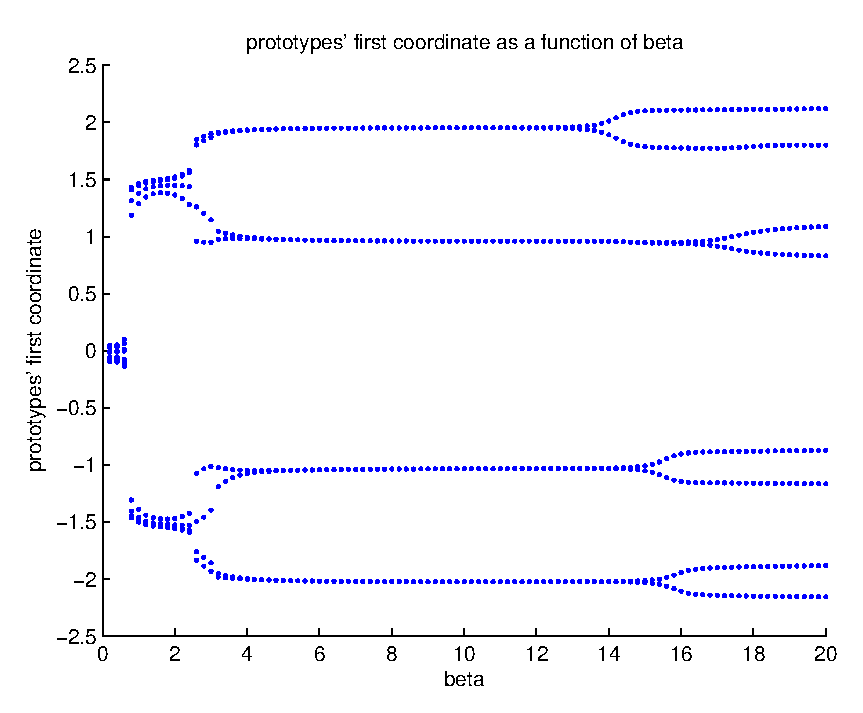
\includegraphics[scale = 0.55]{ex4_soft_kmeans_protbeta}}
\caption{Soft K-means clustering with fixed values of $\beta$. [a] scatter plot of the data and the final prototypes (for different values of $\beta$). [b] First coordinate of the prototypes as a function of $\beta$. }
\label{soft_km}
\end{figure}

Figure~\ref{soft_km_an} shows the results obtained for the second implementation of the algorithm in which annealing is applied.

\begin{figure}[h!]
\centering
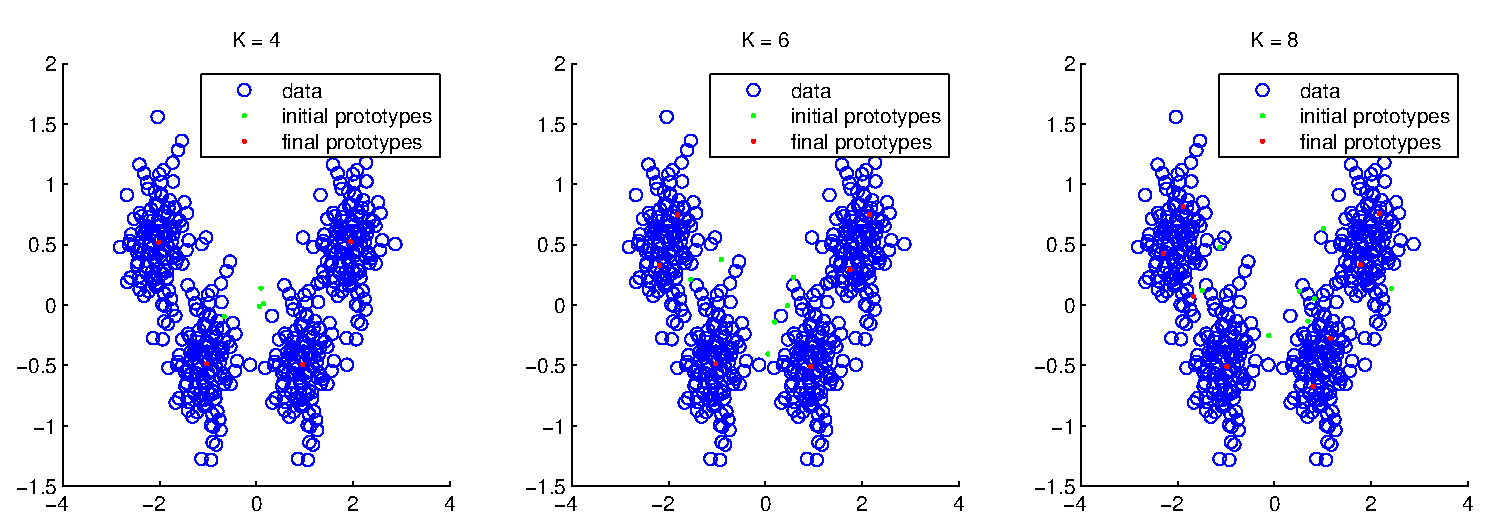
\includegraphics[scale = 0.75]{ex4_soft_kmeans_annealing}
\caption{Soft K-means clustering with annealing for different number of prototypes K.}
\label{soft_km_an}
\end{figure}



\end{document}

